\documentclass[twocolumn,letterpaper,10pt]{IEEEtran}

% common
\usepackage{cite,url,color}
\usepackage{graphicx}
\DeclareGraphicsExtensions{.pdf,.jpeg,.png,.eps}

% math
\usepackage{multirow}
\usepackage{booktabs}
\usepackage[cmex10]{amsmath}
\usepackage{amssymb,bm}
\interdisplaylinepenalty=2500

% algorithm
\usepackage{algpseudocode} % we use this
\newcommand{\algrule}[1][.5pt]{\par\vskip.25\baselineskip\hrule height #1\par\vskip.25\baselineskip}

% subfig
\usepackage[caption=false,font=footnotesize]{subfig}
\usepackage{hyperref}
\hypersetup{
  colorlinks=true,
  linkcolor=black,
  citecolor=black,
  filecolor=black,
  urlcolor=black,
  pdfborder={0 0 0}
}

% theorem
\usepackage[amsmath,thmmarks]{ntheorem}
\newtheorem{theorem}{Theorem}

% my command
\newcommand{\ve}[1]{\mathbf{{#1}}}
\newcommand{\abs}[1]{\ensuremath{\vert #1\vert}}
\newcommand{\norm}[1]{\ensuremath{\Vert #1\Vert}}
\newcommand{\diag}{\ensuremath{\mathrm{diag}}}
%\newcommand{\lby}[1]{\textcolor{red}{#1}} % for reply letter
\newcommand{\lby}[1]{#1} % final version

% correct bad hyphenation here
%\hyphenation{op-tical net-works semi-conduc-tor Chang-sha}

%------------------------------------------------------------------------------

\begin{document}

\title{Title}
\author{%
Benyuan~Liu$^{1,*}$%
\thanks{\textit{Asterisk indicates corresponding author.}}%
\thanks{$^1$B. Liu is with the Department of Biomedical Engineering,
Fourth Military Medical University, Xi'an 710032, China. (e-mail: byliu@fmmu.edu.cn)}
\thanks{Manuscript received \today{}.}%
}

% The paper headers
\markboth{IEEE Trans.}{}
% {Liu \MakeLowercase{\textit{et al.}}: Quantized Compressive Sensing}

\maketitle

%------------------------------------------------------------------------------

\begin{abstract}
\boldmath
In low-power wireless telemonitoring,
physiological signals must be compressed before transmission to extend battery life.
In this paper, we propose a two-stage data compressor based on quantized compressive sensing (QCS),
where signals are firstly compressed by compressive sensing with a 50\% compression ratio
and then quantized with 2-bit per measurement.
We also develop a reconstruction algorithm, called Bayesian De-Quantization (BDQ),
to recover signals from the quantized compressed measurements.
This algorithm exploits both the model of quantization errors and
the correlated structure of physiological signals, which improves the quality of recovery.
We validate the proposed data compressor and the recovery algorithm on a wrist-type photoplethysmography (PPG) data.
This dataset is used to estimate the heart rate during fitness training.
Results show that an average estimation error of 2.596 beats per minute (BPM) is achieved using QCS and BDQ.
This accuracy approaches the performance on non-compressed data,
but we transmit n bits instead of n samples, which is a substantial improvement for low-power telemonitoring.
\end{abstract}
\begin{IEEEkeywords}
    Quantized Compressive Sensing, Block Sparse Bayesian Learning, Data Compression, Telemonitoring
\end{IEEEkeywords}

%------------------------------------------------------------------------------

%---- 1. intro
\section{Introduction}

In wireless health monitoring, hybrid types of physiological signals are collected
from on-body sensors, then these data are transmitted to nearby smart phones or a data central via wireless networks.

\begin{figure}[!htbp]
    \centering
    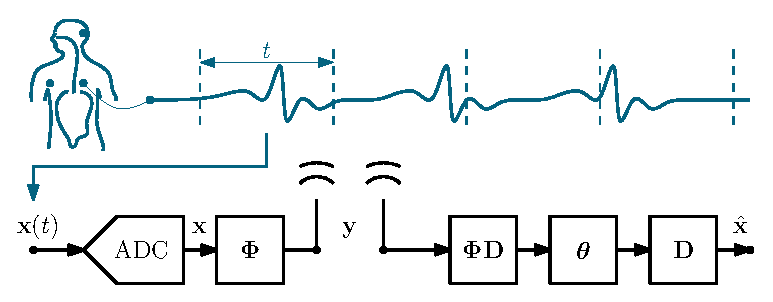
\includegraphics[width=\columnwidth]{diagram}
    \caption{Caption for a figure.}
\end{figure}

The wearable devices are usually battery powered. To reduce the power consumption and extend battery life,
data must be compressed before transmission. liu et, al. \cite{liu2013energy}.

%----
\section*{Acknowledgment}
The authors thank Dr. Hongqi Fan, Dr. Xiaoyi Pan for valuable discussions.
We would also like to thank anonymous reviewers for providing insightful comments.

%----
\ifCLASSOPTIONcaptionsoff
  \newpage
\fi

\bibliographystyle{IEEEtran}
\bibliography{ieee}

%===============================================================================
% biography section
%
% If you have an EPS/PDF photo (graphicx package needed) extra braces are
% needed around the contents of the optional argument to biography to prevent
% the LaTeX parser from getting confused when it sees the complicated
% \includegraphics command within an optional argument. (You could create
% your own custom macro containing the \includegraphics command to make things
% simpler here.)
%\begin{IEEEbiography}[{\includegraphics[width=1in,height=1.25in,clip,keepaspectratio]{mshell}}]{Michael Shell}

%\end{IEEEbiography}
% or if you just want to reserve a space for a photo:

% insert where needed to balance the two columns on the last page with
% biographies
%\newpage

% You can push biographies down or up by placing
% a \vfill before or after them. The appropriate
% use of \vfill depends on what kind of text is
% on the last page and whether or not the columns
% are being equalized.

%\vfill

% Can be used to pull up biographies so that the bottom of the last one
% is flush with the other column.
%\enlargethispage{-5in}

% that's all folks, happy reading!
\end{document}

